\chapter{Voorbereiding} \label{cha:voorbereiding}

\section{Inleiding} \label{sec:inleiding}
Project \projectname is een augmented reality product, in opdracht van \textit{Avans Hogeschool Breda}.

\section{Tools} \label{sec:tools}
De volgende tools zullen worden gebruikt het interaction design te realiseren.

\begin{table}[h]
  \centering
  \caption{Tools}
  \label{tb:table}
  \begin{tabular}{crl}
    \toprule
    Naam     & Type\\
    \midrule
    SketchUp     & 3D modelleer software\\
    Blender  & 3D modelleer software\\
    Adobe Photoshop & grafisch bewerkings programma\\    
    \bottomrule
  \end{tabular}
\end{table}

\newpage
\section{Conceptschetsen} \label{sec:conceptschetsen}
\begin{figure}[h]
  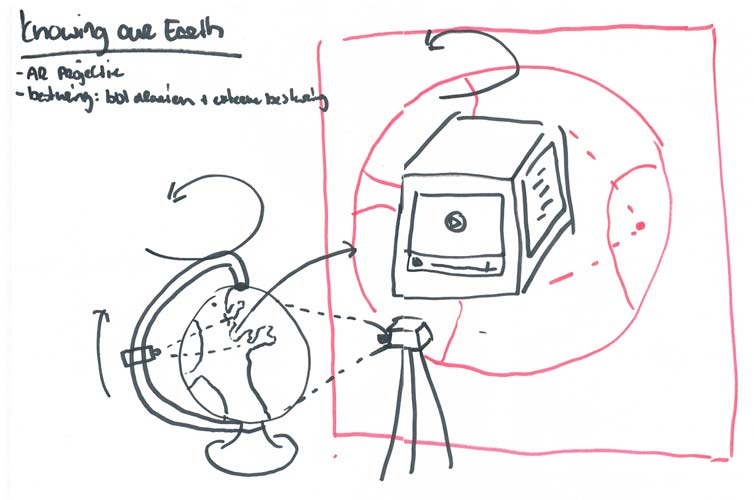
\includegraphics[width=100mm]{figs/concept1.jpg}
  \caption{Concept tekening 1 \textit{(18-April-2014)}}
  \label{fig:concept1}
\end{figure}
\begin{figure}[h]
  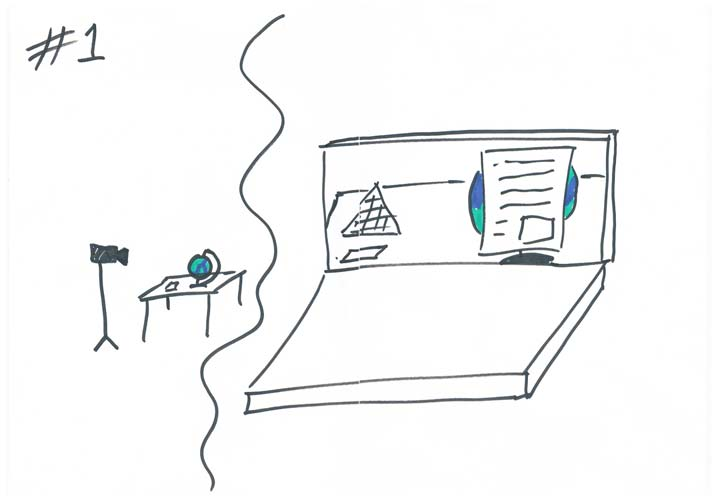
\includegraphics[width=100mm]{figs/concept2.jpg}
  \caption{Concept tekening 2 \textit{(18-April-2014)}}
  \label{fig:concept2}
\end{figure}